\section{Introduction}

Understanding product aspect-sentiments and tracking its changes in a timely manner can support better decision-making for commercial purposes, such as enlightening online retailers to make timely sales plans. Therefore, the \textit{Dynamic Summarization on Product Aspects} task is of great importance. It not only indicates products' dynamic aspect-sentiment changes, but also depicts the changes into readable contexts for easier interpretation.

Prior investigations on another similar topic, review summarization, mainly follow Natural Language Generation (NLG) approaches, such as using new Recurrent Neural Network (RNN) variant that uses gated connections to construct a character-level text generation mode or designing a multi-task model to predict rating and generate review summarization simultaneously using pairwise user-product relationship. Memory network is also used for review summarization generation. 
\begin{figure}  
	% \advance\leftskip-1cm 
	\centering
	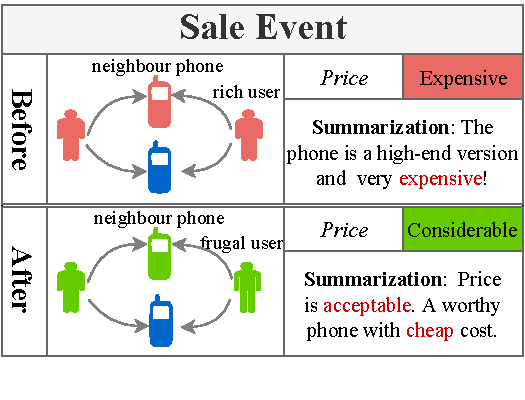
\includegraphics[width=0.8\columnwidth]{img/chapter5/example.pdf}
	% 	\vspace{-1em}
	\caption{An example to illustrate how to dynamically select neighbour products (red phone $\rightarrow$ green phone) for depicting current product (blue phone) sentiment change before \& after a sale event from user behaviors.}
	\label{fig:c5_example}
	% 	\vspace{-1.5em} 
\end{figure}
However, all these models are originally designed for static review summarization and take product reviews as model input. They are vulnerable to depict product sentiment changes because of (real-time review) data sparsity. For instance, after investigating 2.16 billion products sold by \textit{Taobao}, a world-leading online shopping website owned by Alibaba, only 0.05\% of products are able to gather more than 100 reviews within a three-day window. Thus, review-based approaches are not feasible for dynamic summarizations in large scope because of the lack of instant reviews. 

On the other hand, user behavior offers an alternative to address sentiment dynamics. Based on the statistics of the \textit{Taobao} collection, more than 2.53\% of products can receive more than 100 multi-type user behaviors (e.g., \textit{`Click'} or \textit{`Purchase'}) within a three-day window where the coverage is 50 times greater than the review scope. Rational Choice Theory, on the theory side, proves that user shopping behavior rationality has a coherent relationship with the product peculiarity. As Figure \ref{fig:c5_example} depicted, when a sale event on a high-end phone brings frugal users' instant \textit{clicks}, behavior-based algorithms can immediately consume this information and locate updated neighbour products (red phone $\rightarrow$ green phone), whose sufficient reviews help to update the product (blue phone) summarization. For review-based approaches, accumulating enough reviews to characterize this dynamic change may take a longer time. 

In this paper, instead of review summarization, I aim to generate product aspect summarization in a dynamic manner. They are similar topics but still with huge differences in terms of concept definition and generated summary context. Conceptually, review summarization reflects customer subjective and personalized expressions on products. While aspect summarization contains objective descriptions only on restricted product aspects. Contextually, review summarization contains more emotional and general terms in a free format, such as `I love its color so much'. While aspect summarization generates more formal and descriptive expressions, which only focus on specific aspects such as `price is more expensive than expected'. 

Motivated by all mentioned above, I propose a  \textbf{B}ehavior based \textbf{D}ynamic \textbf{S}ummarization (BDS) model to accommodate user behavior for dynamic product aspect summarization. The user shopping preference is stable in a relatively long-term period, which offers us the theoretical feasibility to learn product behavior representation from user dynamic behavior and consistent shopping preference. The learned representation supports neighbor product selection from a group of seed products with abundant instant reviews (\textbf{Task 1}) and meanwhile implicitly helps to generate aspect summarization from product own descriptive phrases and neighbour products' filtered sentimental phrases (\textbf{Task 2}). As both user behavior and seed products' instant reviews are changed across time, the selected neighbour products and generated summarizations are associated with changes as well. The contribution of this work is threefold: 

\begin{itemize}
	\item To the best of my knowledge, this is the first effort to leverage user behavior for dynamic summarization on product aspects. This work pioneers behavior-based summarization investigation.  
	\item In my model, a reinforcement learning approach learns the sampling strategy on seed products with rewards from both sentiment (calculated from behavior-to-sentiment prediction) and semantic (calculated from summarization generation) viewpoints. When generating product aspect summarization, my model does not require target product's reviews as model input, which is able to solve review sparseness, even zero-review, problem.  
	\item  Experiments on a large E-commerce dataset show that my proposed model significantly outperforms the baselines from both automatic and human perspectives. Extensive studies also prove the efficacy of each model input component.   
	
\end{itemize}